\chapter{Dealing with File Bloat}\label{ch:bloat}

\summary{
In Chapter~\ref{ch:floats} we converted the implementation of our previously developed system into one that uses \html{}, \css{}, and JavaScript in place of \gls{pdf} and Adobe Acrobat, which vastly increases its portability. We also added support for floating items, which allows us to produce document layouts that are extremly similar to those used in newspapers, magazines, and academic journals.

In this chapter, we turn around and address the elephant in the room: what effect does the inclusion of all these renderings have upon file size, and what can we do about it?
}

\section{Rationale}
In the system described so far, the emphasis has been firmly upon reducing the computational complexity of layout operations at document view-time, and therefore little consideration has been given to the filesize of the output malleable documents.

%\todo{Put in some pdfdump output comparing ``normal'' pdfs with my malleable ones (maybe as an appendix)}

The tradeoff between filesize and required computation has previously been justified on the basis that storage is cheap,\marginpar{as of 2015, one US dollar will buy around three gigabytes of \textsc{nand} flash memory} light, and small, and that batteries, although relatively inexpensive, already comprise a significant portion of the overall mass and volume of most portable devices that are suitable for reading \ebook{}s. The consequence of this is that adding more storage would have little impact upon devices' aesthetics, but adding extra battery life (emerging nanotube battery technology notwithstanding) would result in vast increases in devices' overall bulk and mass.

Despite this, it seems perverse to make no attempt at all to keep filesizes as small as possible, as long as there are no (or limited) impacts upon the required computation at view-time.

Much like typesetting algorithms, few compression algorithms are designed with the minimisation of computation in mind. Consequently, the result of compressing the data using some generic algorithm is likely to require significantly more computation to decompress than a carefully designed bespoke algorithm. The following section describes work towards such an algorithm.


\section{Implementation}
The most obvious saving that can be made is with the duplication of a document's textual content. The systems described in Chapters \ref{ch:malleable}~and~\ref{ch:floats} both contain as many copies of the document text as there are pre-rendered galleys. In practice, there is no real need for more than one copy to be present in the file. Two approaches to this problem were considered.

\subsection{Pointers into the Source Text}
The first approach to be considered was to include the plaintext source of the document in its entirety, and for each rendering to contain only pointers to the relevant sections of text, instead of the words themselves. These pointers can either be absolute (in the form of a character offset from the start of the text) or logical (in the form \emph{paragraph m, word n}). If the document text is to be included as a plaintext string, absolute pointers are easier to use than logical: logical pointers require either an auxiliary data structure to map the logical pointers to absolute ones, or for the document text to be stored in a format reflecting the logical structure, \ie{} not in plain text.

The principal drawback of using this approach is that on occasion, the output of the linebreaking process does not precisely match the input: for example in the case where words are hyphenated (requiring one word to be broken into two parts, and the addition of a hyphen) or where certain glyphs may be substituted for others (such as with the use of ligatures, where a glyph pair or triplet may be replaced with a single glyph). For this reason, this approach was not considered further.


\subsection{Use of a Dictionary}
\label{sec:dictionary}
The second approach considered was the use of a dictionary to act as a lookup table for each word-level item produced by the linebreaking process.

A document's source text itself is likely to contain significant redundancy. In the 1930s, American linguist George Kingsley Zipf proposed \emph{Zipf's law},\hspace{0pt}\cite{zipf1932} which (broadly) states that given a sizeable sample of text in any given language, the frequency of any word is inversely proportional to its rank in the frequency table. Stated another way, the most common word tends to appear twice as often as the second most common word, three times as often as the third most common word, and so on. There have been many subsequent studies on redundancy in English that have come to related conclusions, for example Claude Shannon estimated the redundancy of written English to be around 50\%.\hspace{0pt}\cite{Shannon1951, Hirst1988}

\begin{sidewaystable} \footnotesize
    \myfloatalign
  \begin{tabular}{rrlrlrlrlrl} \toprule
    & \multicolumn{2}{l}{\textsc{Butterley}} & \multicolumn{2}{l}{\cite{Pinkney2011}} & \multicolumn{2}{l}{\textsc{Shakespeare}} & \multicolumn{2}{l}{\textsc{King James Bible}} & \multicolumn{2}{l}{\textsc{British National Corpus}}\\ 
    \midrule
		& $\numprint{103}$  & the       & $\numprint{233}$  & the      & $\numprint{23197}$  & the & $\numprint{62099}$  & the   & $\numprint{5375304}$  & the  \\ 
		& $\numprint{35}$   & of        & $\numprint{134}$  & of       & $\numprint{19540}$  & I   & $\numprint{38576}$  & and   & $\numprint{3010713}$  & of   \\ 
		& $\numprint{33}$   & and       & $\numprint{116}$  & to       & $\numprint{18263}$  & and & $\numprint{34445}$  & of    & $\numprint{2541227}$  & to   \\ 
		& $\numprint{31}$   & in        & $\numprint{75}$   & and      & $\numprint{15592}$  & to  & $\numprint{13387}$  & to    & $\numprint{2463817}$  & and  \\ 
		& $\numprint{25}$   & to        & $\numprint{75}$   & a        & $\numprint{15507}$  & of  & $\numprint{12735}$  & And   & $\numprint{2015815}$  & a    \\ 
		& $\numprint{23}$   & for       & $\numprint{56}$   & is       & $\numprint{12516}$  & a   & $\numprint{12451}$  & that  & $\numprint{1750205}$  & in   \\ 
		& $\numprint{23}$   & a         & $\numprint{52}$   & be       & $\numprint{10825}$  & my  & $\numprint{12167}$  & in    & $\numprint{949677}$   & that \\ 
		& $\numprint{21}$   & was       & $\numprint{50}$   & in       & $\numprint{9565}$   & in  & $\numprint{9760}$   & shall & $\numprint{924763}$   & is   \\ 
		& $\numprint{19}$   & company   & $\numprint{34}$   & as       & $\numprint{9059}$   & you & $\numprint{9508}$   & he    & $\numprint{838955}$   & was  \\ 
		& $\numprint{17}$   & Butterley & $\numprint{32}$   & document & $\numprint{7831}$   & is  & $\numprint{8932}$   & unto  & $\numprint{816193}$   & for  \\ 
    \midrule
    \textsc{total words}  & $\numprint{1232}$ & & $\numprint{3724}$ & & $\numprint{899595}$ & & $\numprint{821133}$ & & $\numprint{97087700}$ & \\ 
    \midrule
    \textsc{unique words} & $\numprint{628}$  & & $\numprint{1436}$ & & $\numprint{67107}$  & & $\numprint{33446}$  & & $\numprint{1733032}$  & \\ 
    \bottomrule    
  \end{tabular}
  \caption[Word frequencies in various documents]{Top 10 most frequent words in various documents. The total number of words and total unique words are also shown for each document. The data used to produce this table assumes a word is any contiguous block of (case-sensitive) non-whitespace characters; thus, ``\texttt{\textcolor{red}{and}}'' is distinct from ``\texttt{\textcolor{red}{And}}'', and ``\texttt{\textcolor{red}{document}}'' is distinct from ``\texttt{\textcolor{red}{document.}}''. The rationale behind this is that the data produced is more closely representative of a real dictionary of atomic ``words'' to be typeset in a malleable document.}
  \label{tab:wordfreq}
\end{sidewaystable}

\begin{figure}
  \begin{center}
  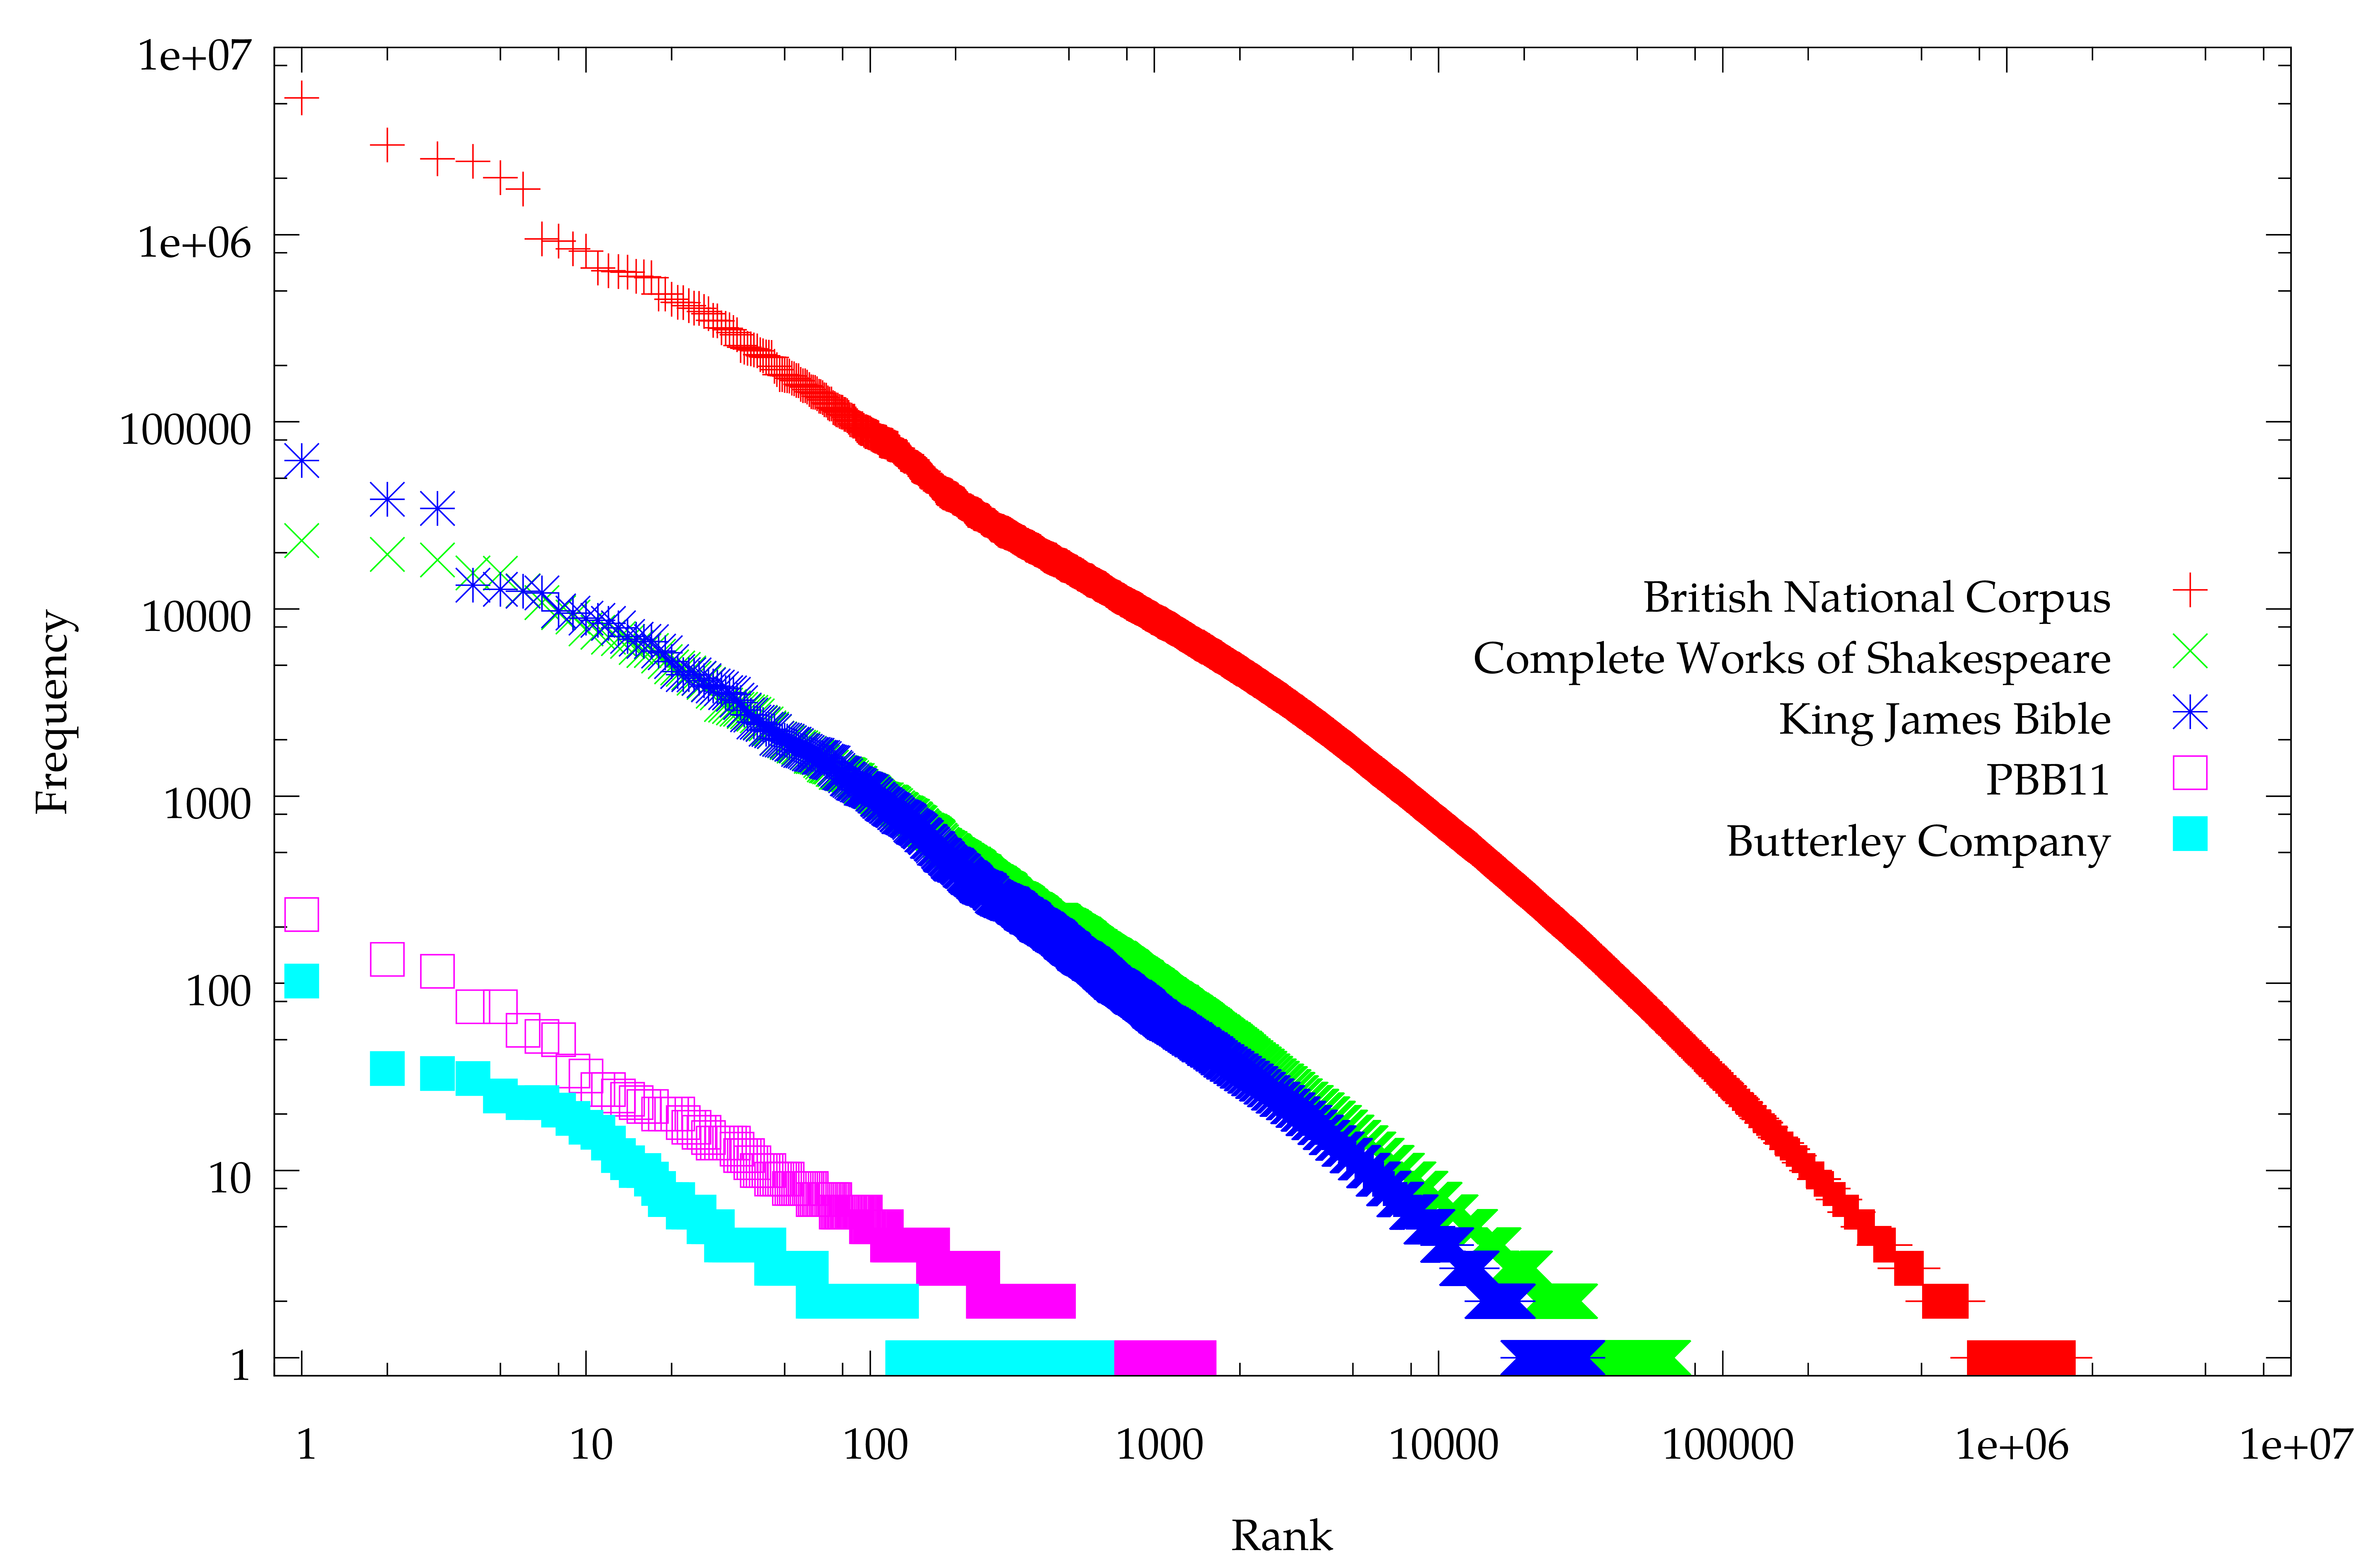
\includegraphics[width=\textwidth]{gnuplot/wordfreq-raster}
  \end{center}
  \caption[Word frequencies in various documents]{Word frequencies in various documents, plotted on a log-log scale. All of these documents, despite their varying lengths, appear to conform well with Zipf's Law, which manifests itself on a log-log scale as a straight line.}
  \label{fig:wordfreq}
\end{figure}

Table~\ref{tab:wordfreq} shows the ten most frequent words in four separate documents and for the British National Corpus\hspace{0pt}\cite{BNCConsortium2007} as a whole.\footnote{The British National Corpus describes itself as \emph{``a 100 million word collection of samples of written and spoken language from a wide range of sources, designed to represent a wide cross-section of British English from the later part of the 20th century, both spoken and written''} and is available freely online at \url{http://www.natcorp.ox.ac.uk/}} The four documents used are the Wikipedia page for the \emph{Butterley Company}\footnote{\url{http://en.wikipedia.org/wiki/Butterley\_Company}}, the author's 2011 paper \emph{Reflowable Documents Composed from Pre-rendered Atomic Components}\hspace{0pt}\cite{Pinkney2011}, the Complete Works of Shakespeare,\marginpar{both Shakespeare and The Bible were obtained as plain text files from Project Gutenberg} and the King James Version of the Bible. Figure~\ref{fig:wordfreq} shows the word frequency data for the same documents plotted on a log-log scale. At the extremities, the data does not conform perfectly to Zipf's Law, though despite their hugely varying lengths, each document does display a clear Zipfian distribution.


This inherent redundancy in natural language can be exploited to produce a simple compression scheme through use of a dictionary. If, for example, the word ``shall'' appears multiple times in a document (in the King James Version of the Bible it appears 9760 times, and in the complete works of Shakespeare 3016 times) it is only stored once in the dictionary. As long as on average (\ie{} over every occurrence of every word) each word's key is lexicographically shorter than the word itself, it can be guaranteed that some redundancy has been removed from the data.

The \gls{html} and JavaScript system described in Chapter~\ref{ch:floats} can be altered to use a dictionary-based lookup table with fairly few modifications. Firstly, since the data for the malleable document must be represented in \gls{json},\footnote{see \url{http://www.json.org/} for full details} some means of including the dictionary must be devised. \gls{json} supports two types of collection. The first is the \emph{object}, which is defined formally as \emph{an \mbox{unordered} set of name/value pairs}. This acts much like an associative array, though it does not guarantee the order of its elements. The second collection type supported by \gls{json} is the \emph{array}, defined as \emph{an ordered collection of values}. Since both must be declared literally (in the forms \texttt{\{\textquotedbl key1\textquotedbl:\textquotedbl word1\textquotedbl,\textquotedbl key2\textquotedbl:\textquotedbl word2\textquotedbl\}} and \texttt{[\textquotedbl word1\textquotedbl,\textquotedbl word2\textquotedbl]} respectively) rather than being populated programatically, using a plain array for the dictionary allows us to omit the keys from the dictionary itself, as they are implied by the order of the elements in the array. Additionally, since this forces the use of integers as keys, the Galley Structure Tree will not require the use of quote marks when the dictionary keys are referenced. If the keys were string values, each use of each key in the Galley Structure Tree would therefore necessitate two extra characters (\eg{} \texttt{\textquotedbl key\textquotedbl} versus \texttt{401}).

It should also be noted that using integers as keys in \gls{json} has different implications to using integers as keys in some more compact binary format. \gls{json} is always stored in some textual encoding (perhaps \textsc{ascii}, perhaps \textsc{utf-8}), and there is no support for numeric representation in any base other than decimal. What might take up one 32 bit integer (\ie{} 4 bytes) in a compiled language such as C might take as many as ten textual characters (10 bytes, assuming that whichever character encoding system is used represents low-\textsc{ascii} characters with only one byte). Conversely, textual representation of integers can be more compact under certain conditions: namely, for values that use three or fewer characters, \ie{} the numbers 0--999.

\begin{figure}
  \begin{center}
  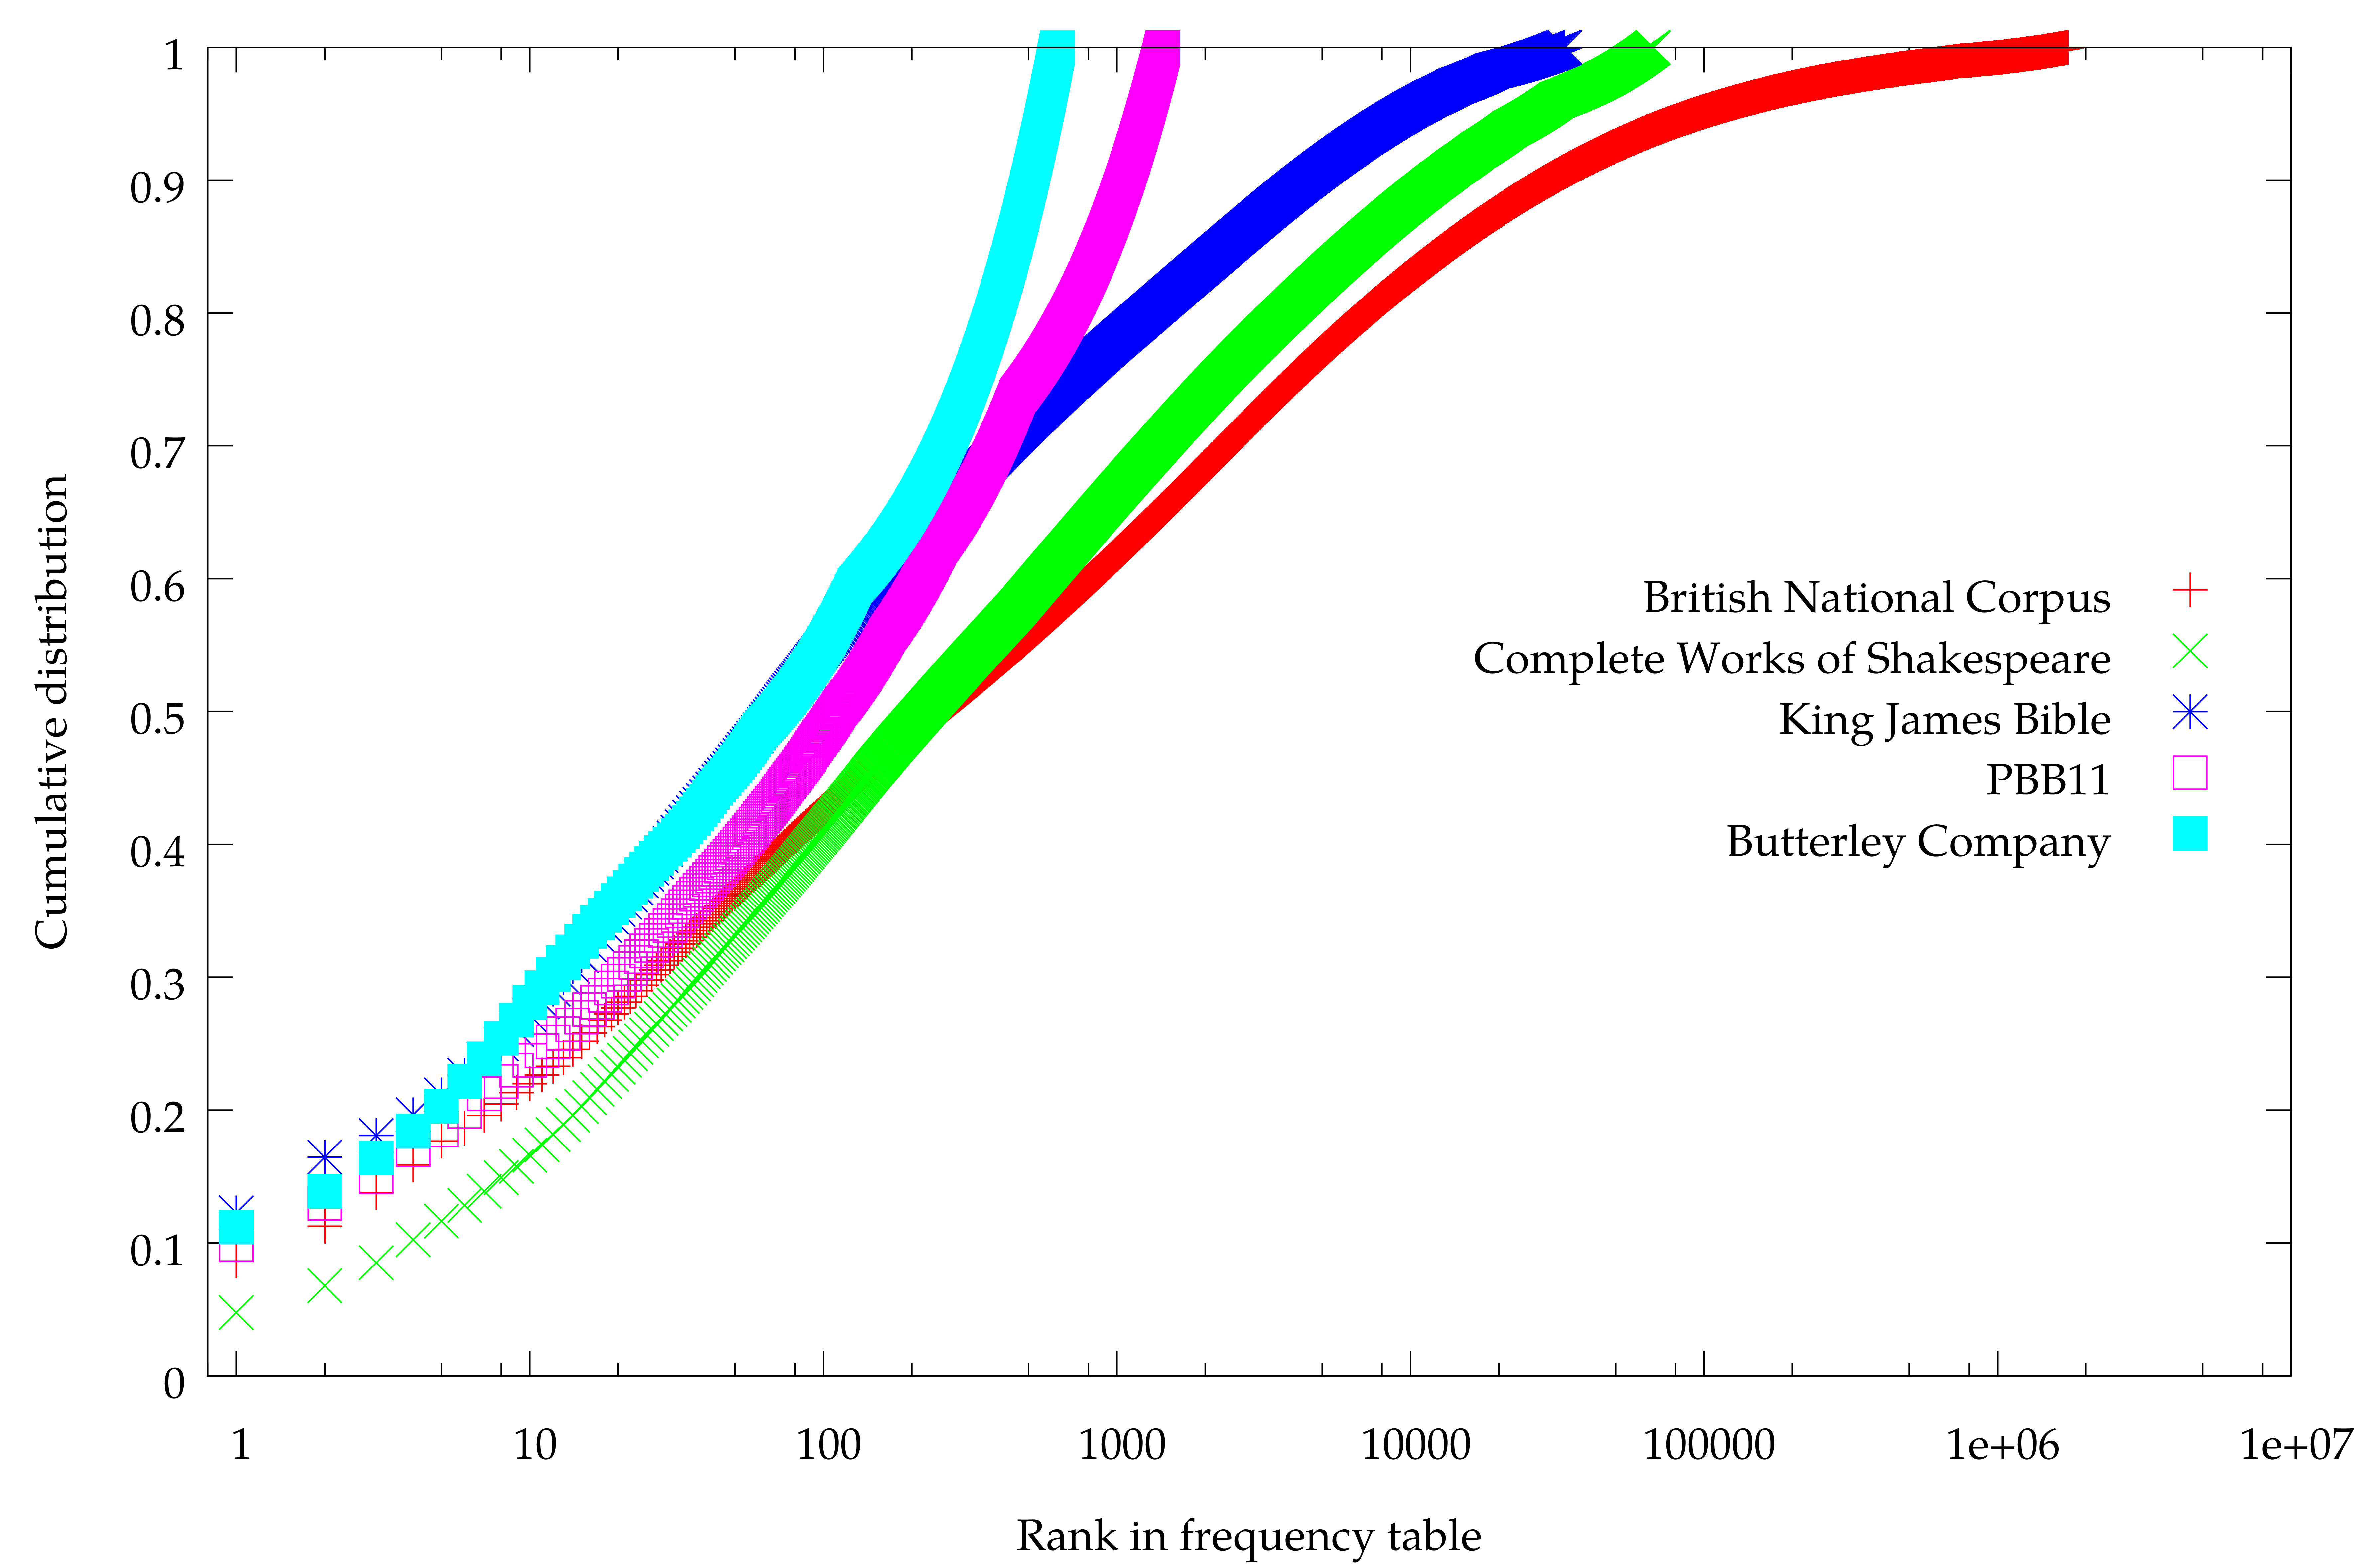
\includegraphics[width=\textwidth]{gnuplot/cumulative-raster}
  \end{center}
  \caption[Cumulative distribution of word frequencies]{Cumulative distribution of word frequencies in various documents. }
  \label{fig:cumulative}
\end{figure}

Referring back to Figure \ref{fig:wordfreq}, to Figure~\ref{fig:cumulative}, and to Zipf's law, it can be seen that even for extremely long documents, the number of words that are ranked in the top 1000 exceeds 60\%, and so as long as the order of words in the dictionary is chosen carefully, using a textual representation of integers can be more compact than a na\"ive binary representation.

It was therefore decided to store the dictionary as an array, ordered such that the most frequently occurring words have the shortest keys.

\subsection{Further Compression Possibilities}
\label{sec:deltas}

The techniques discussed thus far have focused mostly upon exploiting the inherent redundancy in natural language. A fairly large part of the data contained within the Galley Structure Tree has been overlooked: the typesetting data itself.

All of the aforementioned encoding systems have used an absolute value for the x position of each word on each line; that is, each occurrence of each word has an associated value representing the required distance of its placement, in \glspl{point}, from the start of the line. An example of this can be seen in Listing~\ref{lst:datajs} on page~\pageref{lst:datajs}.

With a view to producing data that would be more easily compressible by a generic compression algorithm (that would perhaps be useful if \textsc{HTTP} compression or similar is used to transfer the document data to a device) it was decided to investigate a different approach to storing this data.

In any typeset document, most (if not all) occurrences of the same word will typeset identically upon the page. In particular, the amount of horizontal space reserved for a word will be the same for each occurrence of the word. Similarly, if a document's text is fully justified, the space between words on each individual line will be identical. If the document is left-justified, then each space between each pair of words on \emph{every} line will be identical. This redundancy is present within all the previous encodings, but cannot be picked up by a generic compression algorithm, since it requires knowledge of the typesetting process. By separating the word widths from the spacing, this redundancy can be made more explicit, and therefore easier for a generic compression algorithm to take advantage of.

\begin{lstlisting}[label=lst:deltasdata,captionpos=b,float,language=c,stringstyle=\color{blue},basicstyle=\ttfamily\footnotesize,caption={[Excerpt from a paragraph tree using deltas]Excerpt from a JavaScript data file that uses position deltas in the Galley Structure Tree, representing one galley rendering of one paragraph. The first value in each pair is the position delta (in points) and the second is the dictionary key of the associated word.}]
[
    [[0,982],[3.678,26],[3.678,93]],
    [[0,14],[2.682,1307],[2.682,558]],
    [[0,7],[3.668,557],[3.668,797],[3.668,226]],
    [[0,102],[4.338,9],[4.338,30]],
    [[0,112],[2.4,1013],[2.4,1068]],
    [[0,182],[2.4,1303],[2.4,2],[2.4,547]],
    [[0,308],[15.666,15],[15.666,1114]],
    [[0,177],[2.4,1173],[2.4,229],[2.4,733]],
    [[0,19],[7.336,81],[7.336,26],[7.336,143]],
    [[0,96],[7.116,33],[7.116,97],[7.116,16]],
    [[0,141],[9.444,0],[9.444,30],[9.444,1]],
    [[0,0],[8.78,89],[8.78,8],[8.78,11]],
    [[0,905],[10.008,2],[10.008,0],[10.008,66]],
    [[0,1125],[5.922,5],[5.922,34],[5.922,0],[5.922,1172]],
    [[0,1],[2.676,1053],[2.676,471]],
    [[0,3],[4.008,967],[4.008,112]],
    [[0,524],[10.338,19],[10.338,0]],
    [[0,126],[7.356,571],[7.356,1]],
    [[0,0],[6.896,197],[6.896,16],[6.896,18]],
    [[0,0],[2.4,9],[2.4,5],[2.4,691]],
    [[0,1249],[14.004,1046],[14.004,317]],
    [[0,5],[11.112,289],[11.112,2],[11.112,0]],
    [[0,273],[9.84,24],[9.84,859]],
    [[0,986],[11.34,144],[11.34,210]],
    [[0,263],[2.4,774]]
],
\end{lstlisting}

\begin{lstlisting}[label=lst:deltasdict,captionpos=b,float,language=c,stringstyle=\color{blue},basicstyle=\ttfamily\footnotesize,caption={[Excerpt from a dictionary storing word widths]Excerpt from the dictionary from a JavaScript data file that uses position deltas, where the width of each word is stored alongside the word itself. This is the dictionary from a rendering of \cite{Pinkney2011}: compare its ordering to that shown in Table~\ref{tab:wordfreq} on page~\pageref{tab:wordfreq}.}]
 [["the",14.664],["of",9.996],["to",9.336],["and",17.328],["a",5.328],["is",8.004],["be",11.328],["in",9.336],["as",9.996],["document",47.328],["that",18],["it",6.672],["page",22.656],["for",13.992],["are",14.652],["by",12],["on",12],["will",18.672],["which",29.328],["with",21.336],["this",17.34],["The",18.66],["can",16.656],["an",11.328],["or",9.996],["-",3.996],["eBook",31.332],["used",21.996],["PDF",22.008],["In",9.996],["layout",30],["have",22.656],["from",23.328],["not",15.336],["at",8.664],["width",27.336],["This",21.336],["has",15.996],["then",20.664],["each",21.984],["was",18.66],["typesetting",52.668],["columns",40.668],["simply",32.676],["these",24.66],["text",18],["into",18.672],["hyphenation",59.328],["content",35.328],["quality",33.336],["column",36],["lines",22.668],["only",21.336],["line",18],["ACM",27.336],["our",15.996],["its",11.34],["structure",41.988],["Document",49.992],["penalty",35.328],["between",39.984],["galley",29.328],["order",25.32],["more",24.66],["COGs",30],["out",15.336],["end",17.328],["one",17.328],["use",15.996],["algorithm",46.668],["producing",48.66],["columns.",43.668],["galleys",33.996],["figure",28.656],["simple",32.004],["would",30],
\end{lstlisting}

On the basis of the above observations, the decision was taken that the dictionary should be modified to store the width of each word alongside itself, and that the Galley Structure Tree should be modified so that each word to be typeset is now accompanied by the offset required from the end of the previous word (which will henceforth be referred to as \emph{position deltas}) rather than the absolute offset required from the start of the line. This does of course necessitate two array lookups in the dictionary where previously there would have been one, but since array accesses run in constant time, this does not present a problem. Excerpts from a Galley Structure Tree and dictionary that use this encoding system are shown in Listings \ref{lst:deltasdata}~and~\ref{lst:deltasdict} respectively.

Further redundancy could be removed by exploiting the fact that words tend to be regularly spaced on each line. Whilst the encoding could be modified to allow only regular spacing of words, it was felt that this might be somewhat restrictive, and would detract from the appeal of the system as something that supports complex, arbitrary layouts.

Even without making further compression attempts beyond the encoding system shown in Listings \ref{lst:deltasdata}~and~\ref{lst:deltasdict}\ed the motivation for which, we must remember, was to produce an encoding that was more \emph{compressible}, rather than more \emph{compressed}\ed by pure chance, it turns out that even in its full form, this is the most compact representation yet devised!

\clearpage
\subsection{A Toy Example}
Here we see a very short document represented using each of the aforementioned compression schemes. Each of the following examples produces the dsame output document, which contains two galley renderings of one paragraph: ``This is a short sentence''.

\vspace{0.5in}
This is the original encoding, which uses absolute positioning and no dictionary:

\vspace{0.5in}
\begin{lstlisting}[language=c,stringstyle=\color{blue},basicstyle=\ttfamily\footnotesize]
{
   "galley_widths" : [72, 360],

   "paragraph_tree": [
      [
         [
            [
               [0, "This"], [38.538, "is"], [65.328, "a"]
            ],
            [
               [0, "short"], [51.276, "sen-"]
            ],
            [
               [0, "tence."]
            ]
         ],
         [
            [
               [0, "This"], [22.872, "is"], [33.9, "a"], [44.04, "short"], [71.964, "sentence."]
            ]
         ]
      ]
   ]
}
\end{lstlisting}

\clearpage

This encoding uses a dictionary, which reduces redundancy by avoiding repetition of words. Since this document is so short, all its dictionary keys are the same length. For this reason, its corresponding version using an ordered dictionary (the next level of encoding devised) would be identical and is therefore omitted from this example.

\vspace{0.5in}
\begin{lstlisting}[language=c,stringstyle=\color{blue},basicstyle=\ttfamily\footnotesize]
{
   "galley_widths" : [72, 360],

   "paragraph_tree": [
      [
         [
            [
               [0, 0], [38.538, 1], [65.328, 2]
            ],
            [
               [0, 3], [51.276, 4]
            ],
            [
               [0, 5]
            ]
         ],
         [
            [
               [0, 0], [22.872, 1], [33.9, 2], [44.04, 3], [71.964, 6]
            ]
         ]
      ]
   ],
   "dictionary": ["This", "is", "a", "short", "sen-", "tence.", "sentence."]
}
\end{lstlisting}

\clearpage

This encoding uses a dictionary that also contains the widths of words, so each word in the paragraph tree needs to store only its offset from the end of the preceding word.

\vspace{0.5in}
\begin{lstlisting}[language=c,stringstyle=\color{blue},basicstyle=\ttfamily\footnotesize]
//Ordered dictionary with position deltas
{
   "galley_widths" : [72, 360],

   "paragraph_tree": [
      [
         [
            [
               [0, 1], [19.134, 2], [19.134, 3]
            ],
            [
               [0, 0], [26.82, 6]
            ],
            [
               [0, 5]
            ]
         ],
         [
            [
               [0, 1], [3.468, 2], [3.468, 3], [3.468, 0], [3.468, 4]
            ]
         ]
      ]
   ],

   "dictionary": [
      ["short",     24.456],
      ["This",      19.404],
      ["is",         7.656],
      ["a",          6.672],
      ["sentence.", 46.368],
      ["tence.",    29.628],
      ["sen-",      20.724]
   ]
}
\end{lstlisting}


\clearpage
\section{Results}

The following pages show the evolution of the encoding system, and how the filesizes vary according to the number of included galley renderings, for the same sample documents that are used for Figures \ref{fig:wordfreq}~and~\ref{fig:cumulative}:

\begin{itemize}

 \item Figure~\ref{fig:size-json} (page~\pageref{fig:size-json}) shows the ``original'' encoding system described in Chapter~\ref{ch:floats}, which does not make any attempt to minimise filesize.

 \item Figure~\ref{fig:size-unord} (page~\pageref{fig:size-unord}) shows the encoding system described in Section~\ref{sec:dictionary}, using a dictionary ordered such that the earliest occurring words have the shortest keys. (The dictionary is therefore described as \emph{unordered}.)

 \item Figure~\ref{fig:size-ord} (page~\pageref{fig:size-ord}) shows the encoding system described in Section~\ref{sec:dictionary}, using a dictionary ordered such that the most frequently occurring words have the shortest keys. (The dictionary is therefore described as \emph{ordered}.)

 \item Figure~\ref{fig:size-deltas} (page~\pageref{fig:size-deltas}) shows the encoding system described in Section~\ref{sec:deltas}, which not only uses a dictionary ordered such that the most frequently occurring words have the shortest keys, but also stores the width of each word in the dictionary, so that the Galley Structure Tree contains deltas rather than absolute positioning data.

 \item Figure~\ref{fig:size-all-b} (page~\pageref{fig:size-all-b}) shows a comparison of the filesizes produced by all encodings, and Figure~\ref{fig:size-all-gz} (page~\pageref{fig:size-all-gz}) shows the resultant filesizes when each rendering is further compressed with \texttt{gzip}.
\end{itemize}


\begin{figure}
  \begin{center}
  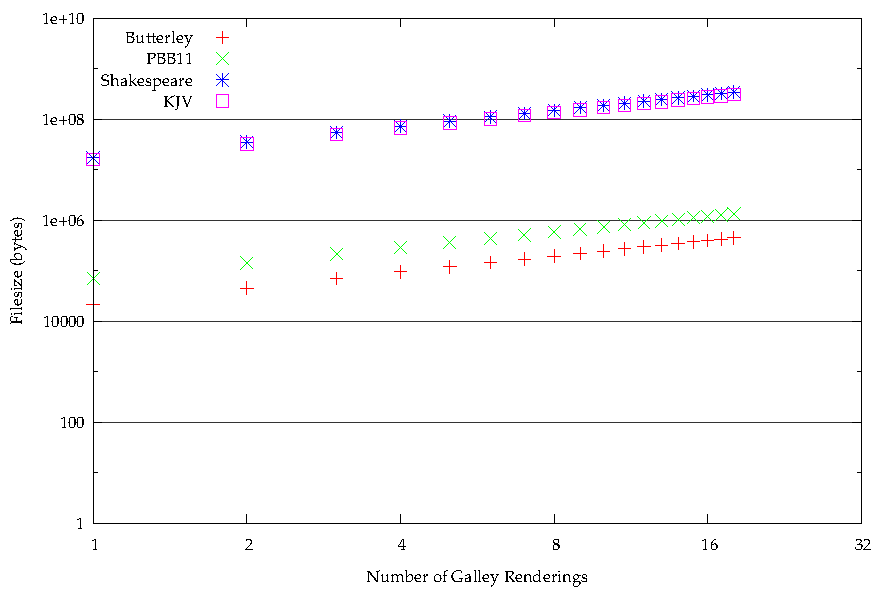
\includegraphics[width=\textwidth]{gnuplot/2-b}
  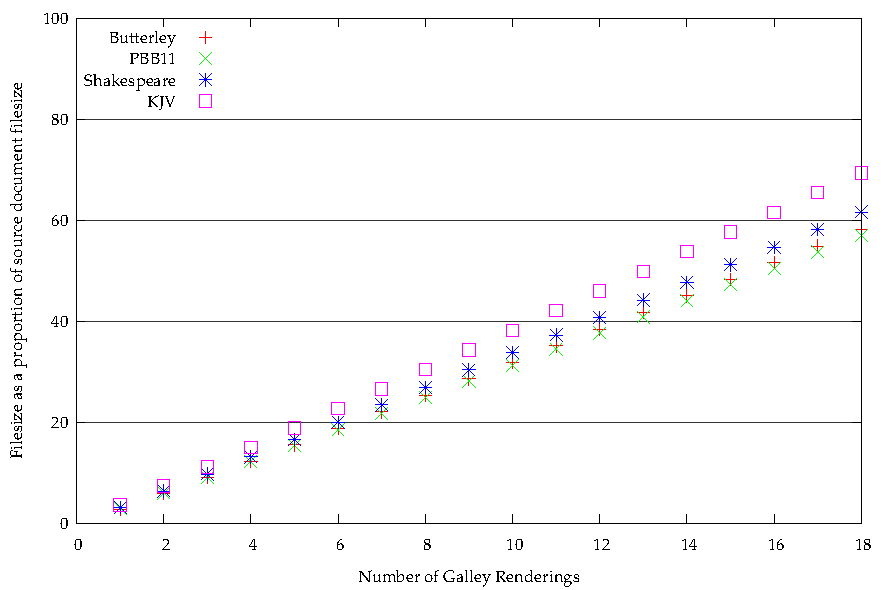
\includegraphics[width=\textwidth]{gnuplot/2-s}
  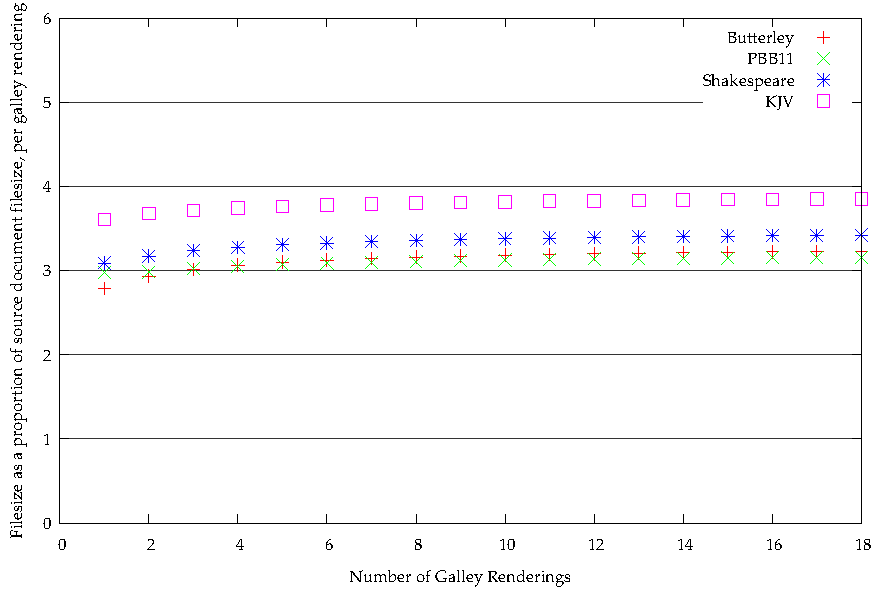
\includegraphics[width=\textwidth]{gnuplot/2-r}
  \end{center}
  \caption[Filesizes of documents in original encoding]{Filesizes of various documents, using the original encoding.}
  \label{fig:size-json}
\end{figure}



\begin{figure}
  \begin{center}
  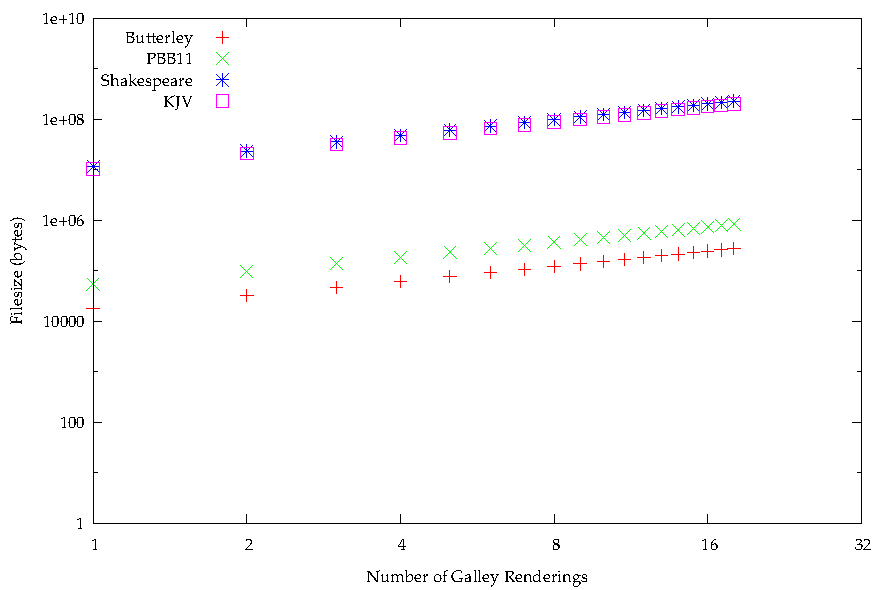
\includegraphics[width=\textwidth]{gnuplot/3-b}
  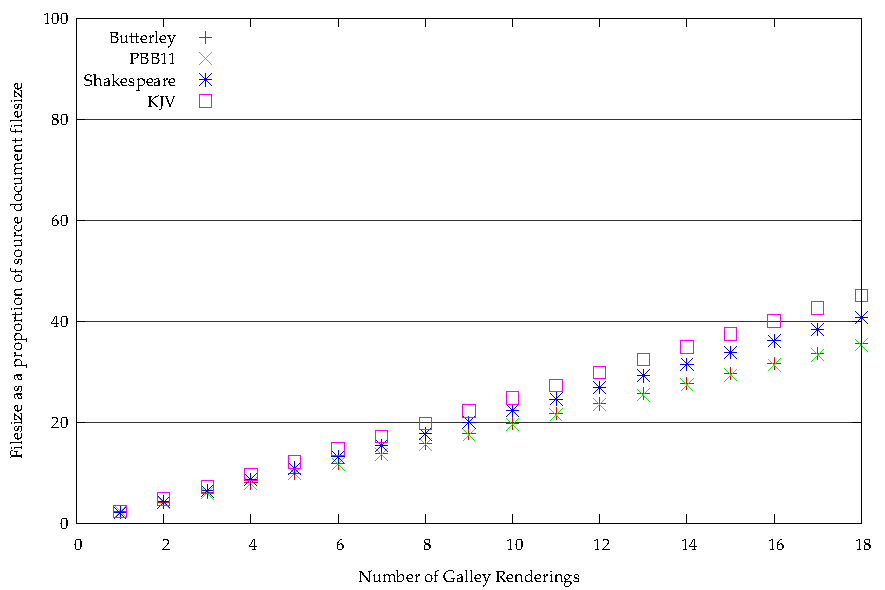
\includegraphics[width=\textwidth]{gnuplot/3-s}
  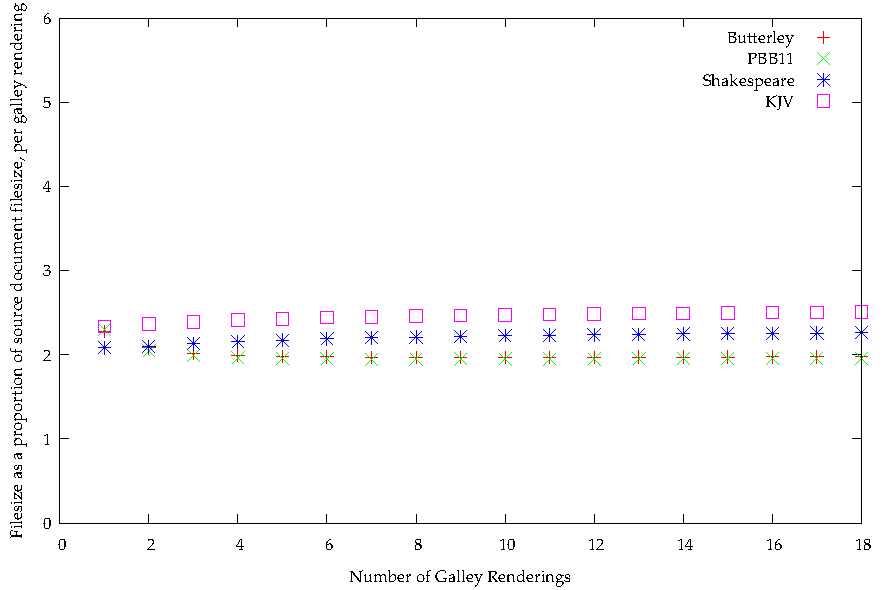
\includegraphics[width=\textwidth]{gnuplot/3-r}
  \end{center}
  \caption[Filesizes with an unordered dictionary]{Filesizes of various documents, encoded using an unordered dictionary.}
  \label{fig:size-unord}
\end{figure}



\begin{figure}
  \begin{center}
  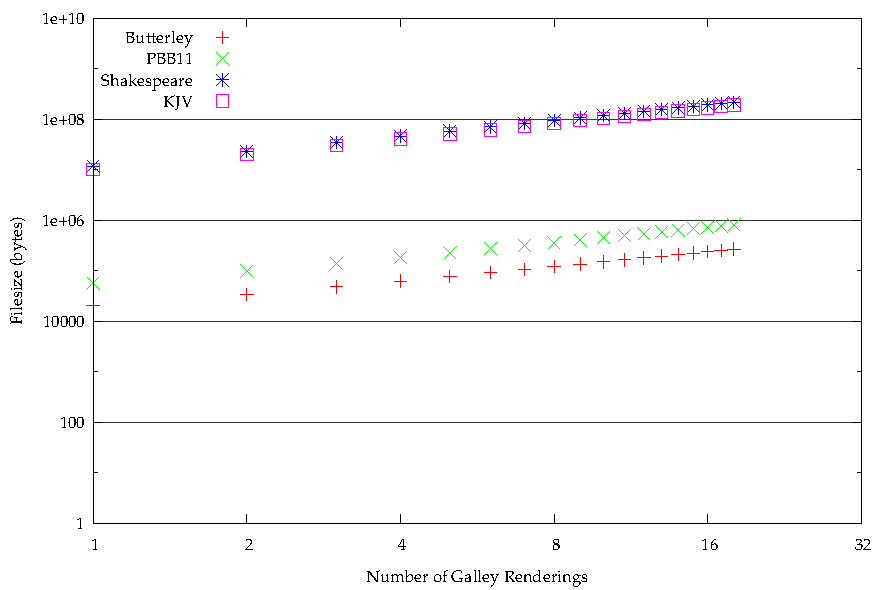
\includegraphics[width=\textwidth]{gnuplot/4-b}
  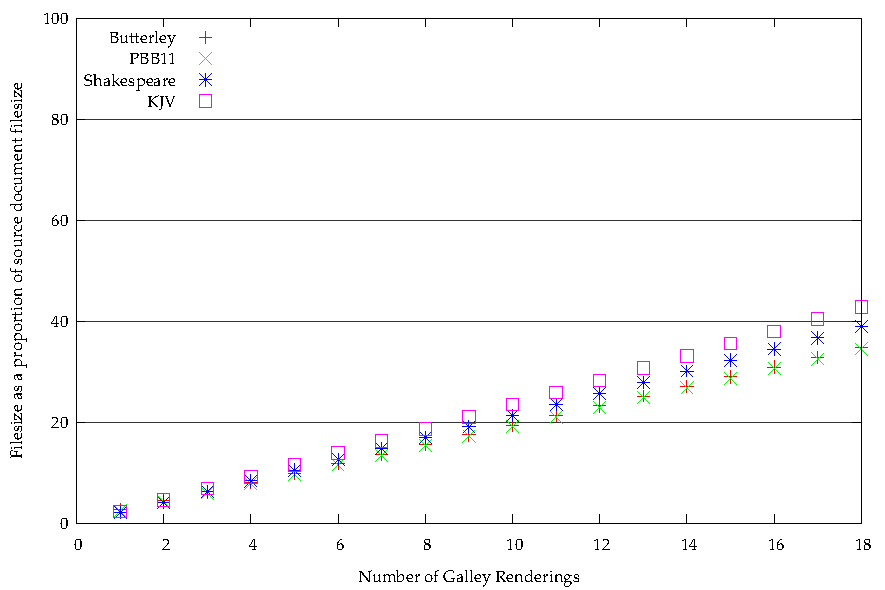
\includegraphics[width=\textwidth]{gnuplot/4-s}
  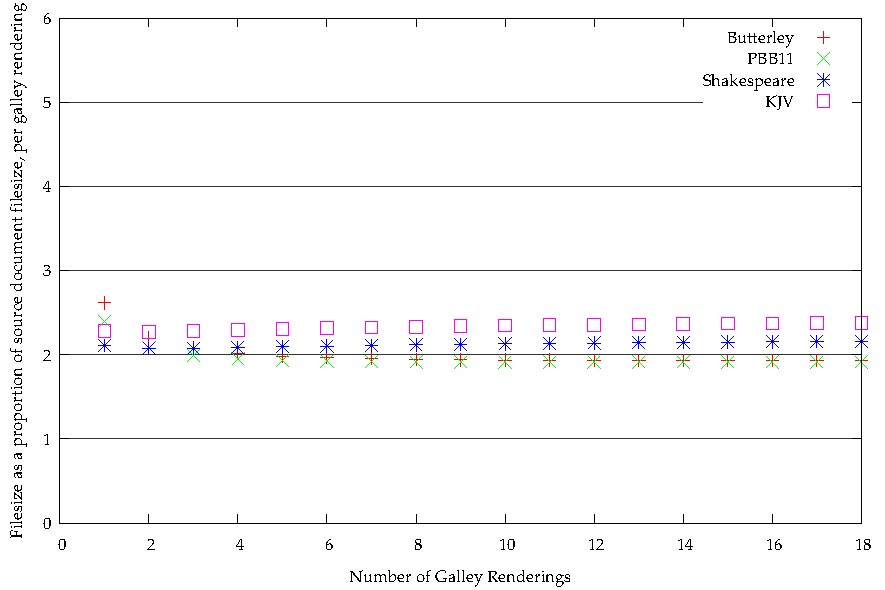
\includegraphics[width=\textwidth]{gnuplot/4-r}
  \end{center}
  \caption[Filesizes with an ordered dictionary]{Filesizes of various documents, encoded using an ordered dictionary.}
  \label{fig:size-ord}
\end{figure}



\begin{figure}
  \begin{center}
  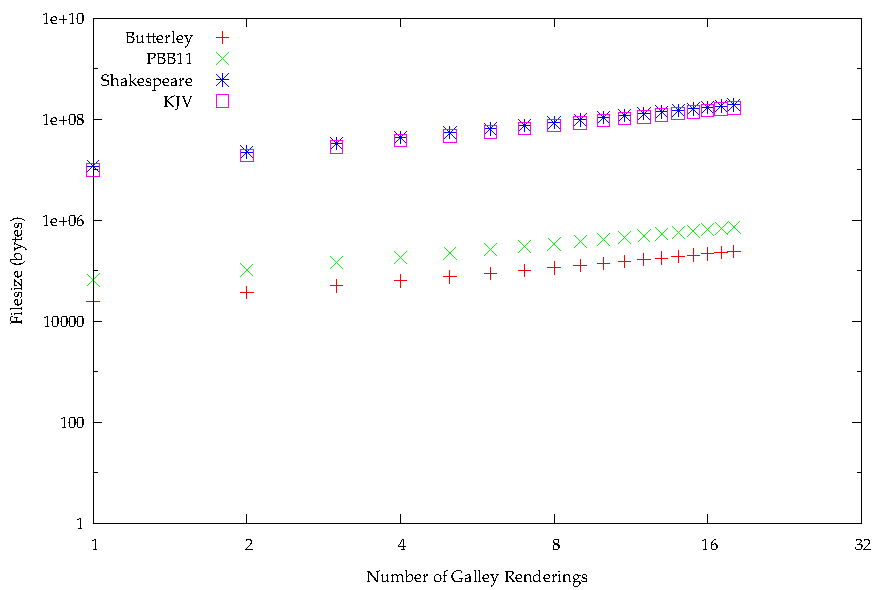
\includegraphics[width=\textwidth]{gnuplot/5-b}
  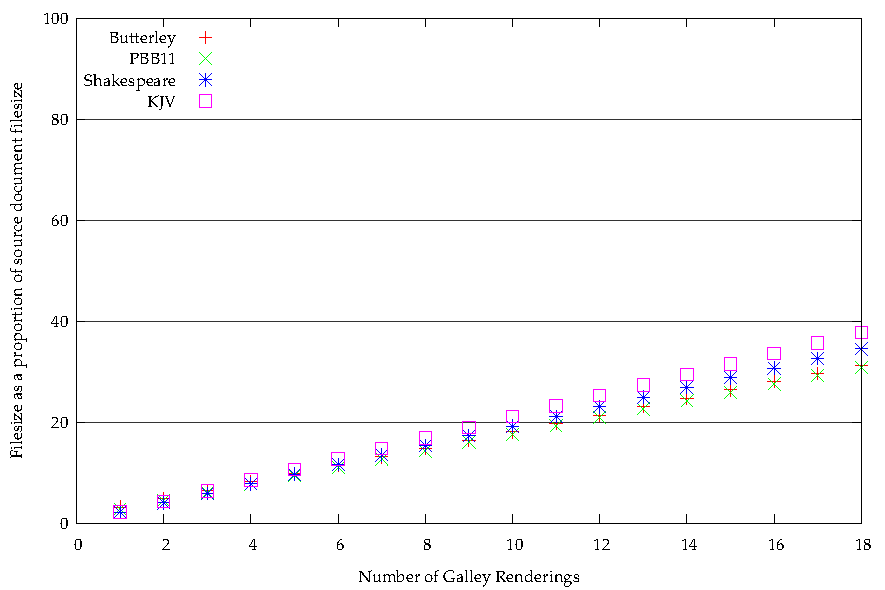
\includegraphics[width=\textwidth]{gnuplot/5-s}
  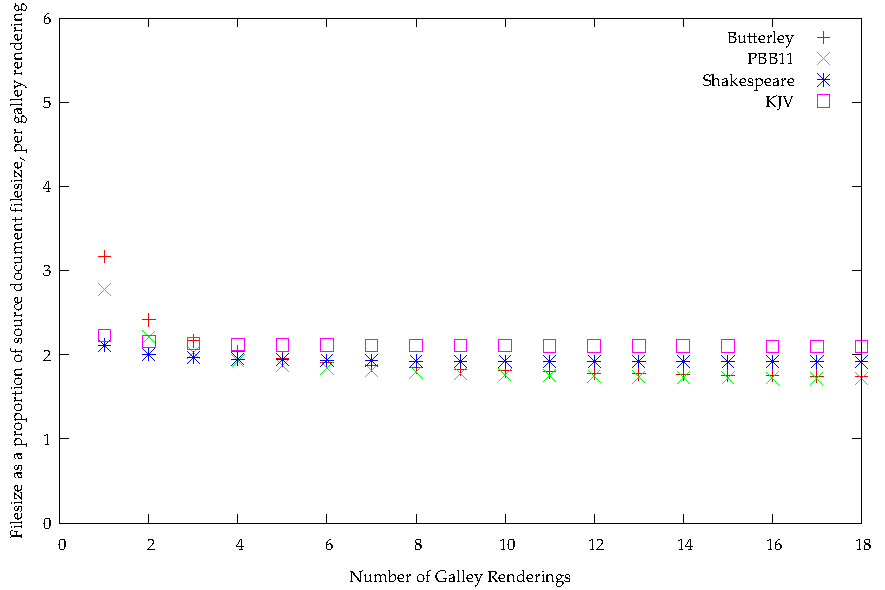
\includegraphics[width=\textwidth]{gnuplot/5-r}
  \end{center}
  \caption[Filesizes with relative positioning]{Filesizes of various documents, encoded using an ordered dictionary with word widths, and position deltas in the Galley Structure Tree.}
  \label{fig:size-deltas}
\end{figure}



\begin{sidewaysfigure}
  \begin{center}
  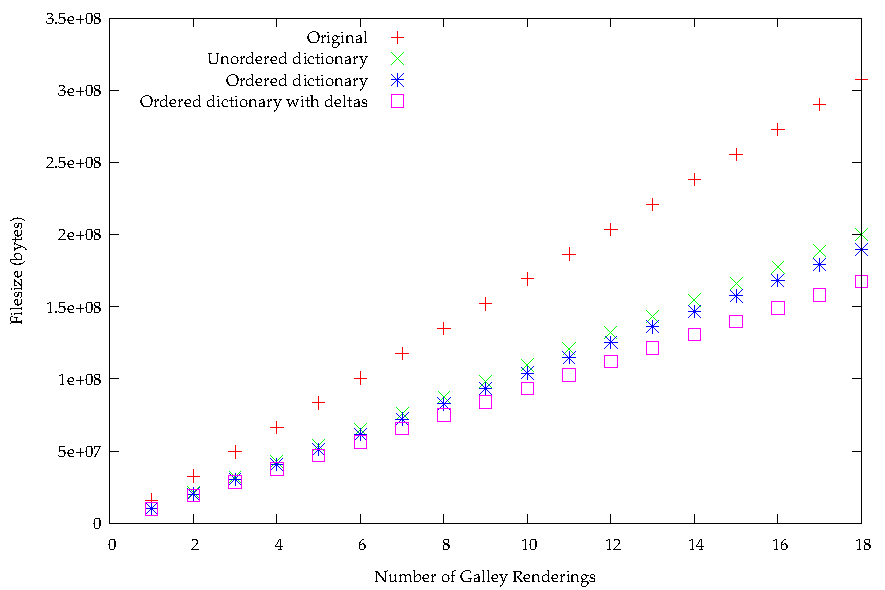
\includegraphics[height=0.5\textheight]{gnuplot/kjv-b}
  \end{center}
  \caption[Comparison of filesizes from all encodings]{A comparison of filesizes produced by all encodings, using the King James Version of the Bible as a sample document.}
  \label{fig:size-all-b}
\end{sidewaysfigure}

\begin{sidewaysfigure}
  \begin{center}
  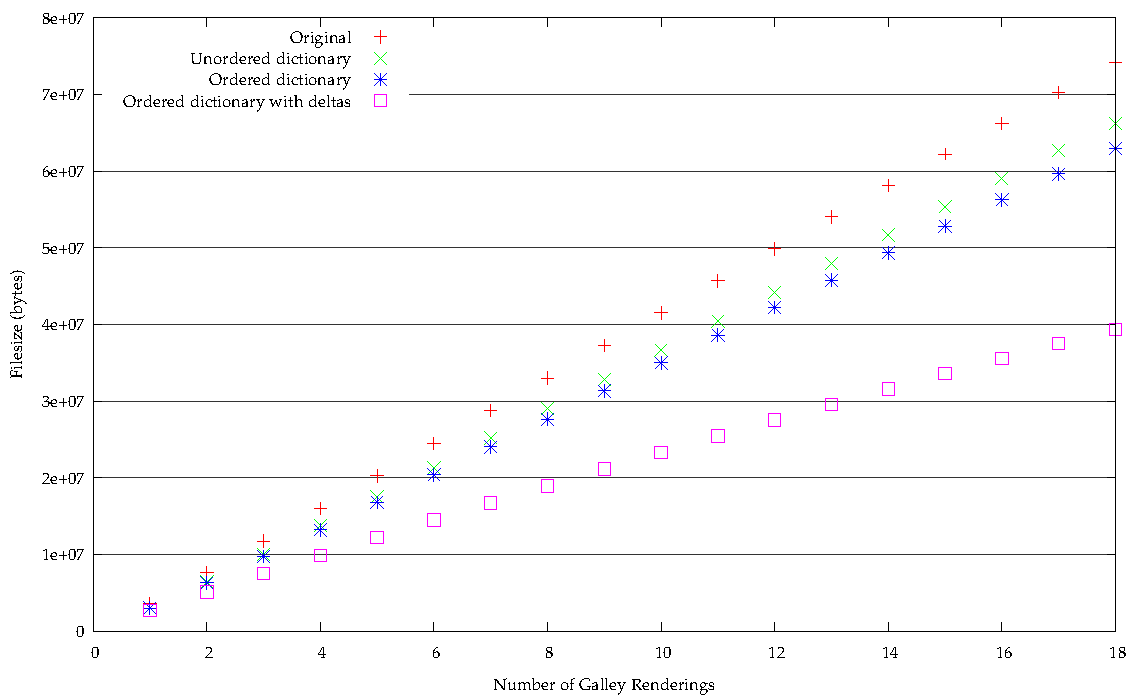
\includegraphics[height=0.5\textheight]{gnuplot/kjv-gz}
  \end{center}
  \caption[Comparison of gzips of all encodings]{A comparison of filesizes of all encodings after gzipping, using the King James Version of the Bible as a sample document. Note the substantial improvement in compression of the encoding that uses position deltas, over the variants that use absolute positioning.}
  \label{fig:size-all-gz}
\end{sidewaysfigure}


% \begin{table}
%     \myfloatalign
%   \begin{tabularx}{\textwidth}{lXXXXXX} %\toprule
%     & \multicolumn{2}{l}{\textsc{source text}} & \multicolumn{2}{l}{\textsc{orig. scheme}} & \multicolumn{2}{l}{\textsc{dictionary}} \\
%     & \textsc{plain} & \textsc{gz} & \textsc{plain} & \textsc{gz} & \textsc{plain} & \textsc{gz} \\ \midrule
%     PBB11~\cite{Pinkney2011} & 23\textsc{k} & 9.4\textsc{k} & 627\textsc{k} & 145\textsc{k} & 314\textsc{k} & 111\textsc{k} \\ \midrule
%     King James Bible & 4.3\textsc{m} & 1.4\textsc{m} & 144\textsc{m} & 32\textsc{m} & 73\textsc{m} & 24\textsc{m} \\ 
%     \bottomrule
%   \end{tabularx}
%   \caption[Comparison of filesizes]{Comparison of filesizes using various encoding methods}  \label{tab:filesize}
% \end{table}


\clearpage


\subsection{Discussion}

It is fairly clear from the preceding graphs that so long as some thought is put in, a lot of redundancy can be squeezed out of the data, without the need to resort to aggressive compression methods that require significant computation during decompression.

Nevertheless, Figures \ref{fig:size-all-b}~and~\ref{fig:size-all-gz} suggest that a significant amount of redundancy remains in each of the encoding schemes: on gzipping, the filesizes are reduced by some 66--75\%. Some of this can be attributed to \gls{json}'s syntax, but it is likely that the blame lies more with the data itself. The dictionary itself is not particularly compact. No advantage is taken of words that share common substrings, nor of words that have identical widths.
Algorithms that do take advantage of substrings, for example \textsc{lz77},\hspace{0pt}\cite{Ziv1977} tend not to have been designed with fast decompression in mind. It is vital that the complexity of any required decompression does not dominate that of the layout process itself.

A further manner in which the data could be compressed is to take advantage of the fact that the values of the position deltas are often repeated, particularly when lines have even spacing between words, which is in the vast majority of cases. This can be seen fairly clearly in Listing~\ref{lst:deltasdata} on page~\pageref{lst:deltasdata}. A second ``dictionary'' can be created in which to store these position deltas. Informal experimentation has suggested this would reduce filesizes by a further 10--15\%, and gzipped filesizes by a further 5\%.

\section{Summary}

The result of the work in this chapter is a reasonably compact version of the document representation model developed in Chapter~\ref{ch:floats}. As an example, a 7-galley malleable version of the King James Bible in the original representation was around 150~\textsc{mb}, and in the most compact representation around 57~\textsc{mb}. This is still considerably larger than the source document (around 4.3~\textsc{mb} as plain text) but does contain data that allows the content to be typeset to seven different widths. The graphs in Figure~\ref{fig:size-deltas} show that each included rendering contributes approximately twice the size of the original plaintext source.

Since the compression used relies entirely on array lookups, the computational overhead for decompression is kept to a minimum. Dealing with moderately larger file sizes seems a reasonable price to pay.
